\chapter{Materials And Methods}
\section{HC18 Dataset}
\subsection{Description}
\label{subsection:dataset}
\noindent

	The collection of 1334 2D ultrasound images of fetal head were collected from the database of the Department of Obstetrics of the Radboud University Medical Center, Nijmegen, the Netherlands. All of the fetal head ultrasound images for this challenge were captured on the standard plane which is the specifically used to measure the HC \cite{thomas}.
	
	The data is split-off into two different subsets. The first one is the training set (including 999 images) which is used for training and validating the model. The other one (including 335 images) is used for a separate testing by submitting to \href{https://hc18.grand-challenge.org/}{Grand Challenge} in order to compare our model with others.
	
%	The size of each 2D ultrasound image is 800x540 pixels with a pixel size ranging from 0.052 to 0.326 mm. The information about the pixel of each image can be found in the CSV format files: ‘training-set-pixel-size-and-HC.csv’ and ‘test-set-pixel-size.csv’. The variability of pixel size resulted from the adjustment of sonographers during examinations which led to a different shape and size of the fetal heads. 
	
	The size of each 2D ultrasound image is 800x540 pixels with a pixel size ranging from 0.052 to 0.326 mm. In addition, each ultrasound image in the training set is accompanied by a manual annotation image. All of the image file-names start with a number. However, the file name only sets up to 805 because some images come from the same examination (different frame during monitoring), therefore they have a similar appearance \cite{thomas}.
	
	\begin{figure}[H]
		\centering
		\subcaptionbox{A fetal head ultrasound image.}{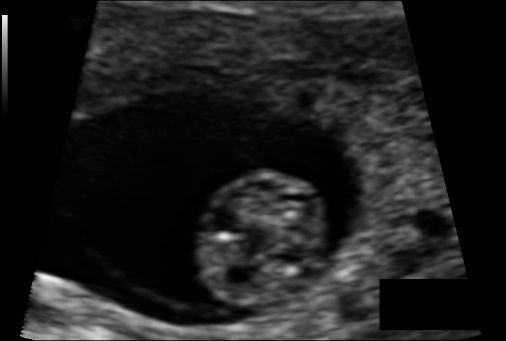
\includegraphics[width=0.45\textwidth]{./hinhanh/chap3/us_image.png}}%
		\hfill % <-- Seperation
		\subcaptionbox{An annotation  created by sonographers.}{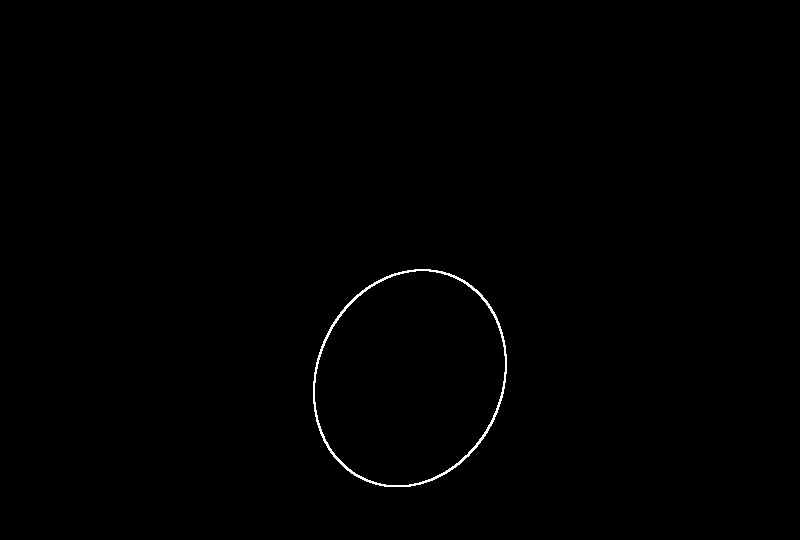
\includegraphics[width=0.45\textwidth]{./hinhanh/chap3/ori_annotation.png}}%
		\hfill % <-- Seperation
		\caption{HC-18 dataset sample.}
		\label{fig:us_image}
	\end{figure}

	
\subsection{Pre-processing}
\label{subsection:preprocess}
\noindent

	During each examination, the sonographer manually drew an ellipse which best fit the fetal head and saved it as an annotation of the ultrasound image. And based on these annotations, we applied a little image processing to extract the ellipse coordinates and created a dataset in COCO format for further training methods.
	
	\begin{figure}[H]
		\centering
		\subcaptionbox{a processed annotation}{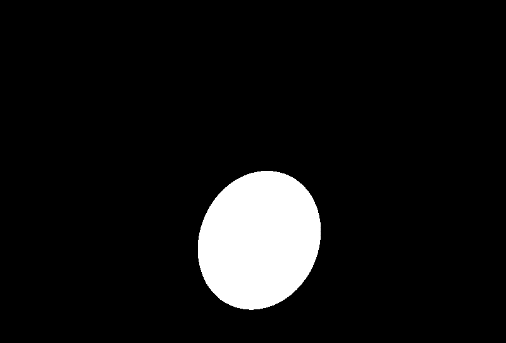
\includegraphics[width=0.45\textwidth]{./hinhanh/chap3/processed_annotation.png}}
		\caption{This annotation is made for Mask R-CNN model.}
		\label{fig:processed_annotation}
	\end{figure}
	
	And then we save it in json file - ”annotations.json” with the information structure including images, categories, and annotations.

	\textbf{Images:}
\begin{itemize}
	\item File name and ID.
	\item Height and width: size of each image.
\end{itemize}

	\textbf{Categories:}
\begin{itemize}
	\item Super-category: name for group of objects (for example: fish – which include lots of fish species).
	\item ID and name
\end{itemize}

	\textbf{Annotations:}
\begin{itemize}
	\item Segmentation: coordinates of annotated pixels (contour).
	\item Area: ground true binary mask.
	\item Is crowd: one or multiple objects in the image.
	\item Image ID, ID, category ID.
	\item Bounding box: offset values.
\end{itemize}
	
	
\section{An Automatic System}
\label{section:proposed_system}
\noindent

	Generally, four main problems are determined in order to estimate fetal head circumference: detection, segmentation, ellipse fitting, and circumference estimation. In which, detection task is to detect the position of the fetal head in the ultrasound image. Segmentation task is to partition or generate a mask surrounding the object on ultrasound image. Ellipse fitting and circumference estimation tasks are drawing a complete ellipse based on the generated mask and calculating the circumference of that ellipse. By adopting Mask RCNN, both detection and segmentation tasks have been solved simultaneously. After that, the Contour-finding, the Ellipse-specific algorithms, and the Ramanujan’s approximation are applied to estimate the fetus head circumference.	
	